\section{Proof of the Limit $\displaystyle \lim_{\theta \to 0} \frac{\sin \theta}{\theta} = 1$}
\label{appendix:lim}
\begin{theorem}
\[ \lim_{\theta \to 0} \frac{\sin \theta}{\theta} = 1 \]
\end{theorem}

\begin{proof}
Assume first that $\theta$ lies between $0$ and $\pi/2$. Figure 1 shows a sector of a circle with center $O$, central angle $\theta$, and radius $1$. $BC$ is drawn perpendicular to $OA$. By the definition of radian measure, we have arc $AB = \theta$. Also $|BC| = |OB|\sin\theta = \sin\theta$. From the diagram we see that
\[ |BC| < |AB| < \text{arc } AB \]

\begin{center}
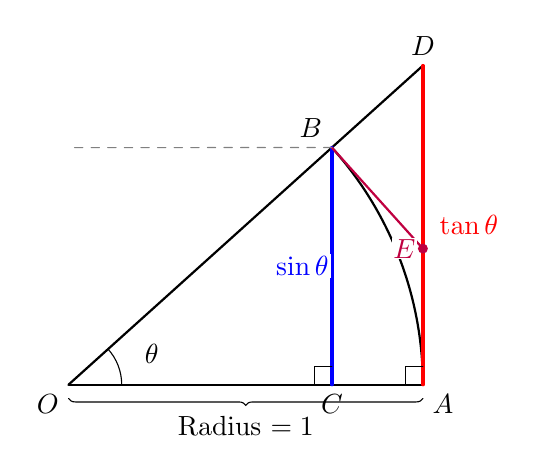
\begin{tikzpicture}[scale=4.5, cap=round, >=latex]
    % --- Definitions ---
    \def\angle{42} % Angle theta (Large enough to see clearly)
    \coordinate (O) at (0,0);
    \coordinate (A) at (1,0);
    \coordinate (B) at (\angle:1); 
    \coordinate (C) at ({cos(\angle)},0); 
    \coordinate (D) at (1,{tan(\angle)}); 
    
    % E is intersection of tangents
    % y_E = tan(theta/2)
    \coordinate (E) at (1, {(1-cos(\angle))/sin(\angle)}); 

    % --- Geometry Drawing ---
    
    % 1. The Main Sectors/Lines
    \draw[thick] (O) -- (D); % Radius extended to D
    \draw[thick] (O) -- (A); % Radius OA
    \draw[thick] (1,0) arc (0:\angle:1); % Arc AB
    
    % 2. Vertical Lines
    \draw[very thick, red] (A) -- (D); % Tangent AD
    \draw[very thick, blue] (B) -- (C); % Sine BC
    
    % 3. Tangent Segment BE
    \draw[thick, purple] (B) -- (E); 

    % 4. Dashed Projection for clarity (Optional but helps depth)
    \draw[dashed, gray] (B) -- (0, {sin(\angle)}); 

    % --- Labels with White Backgrounds to prevent overlap ---
    
    % Dimensions
    \node[red, right] at (1.02, {tan(\angle)/2}) {$\tan \theta$};
    \node[blue, left, fill=white, inner sep=1pt] at ({cos(\angle)}, {sin(\angle)/2}) {$\sin \theta$};
    
    % Points
    \node[below left] at (O) {$O$};
    \node[below] at (C) {$C$};
    \node[below right] at (A) {$A$};
    \node[above left] at (B) {$B$};
    \node[above] at (D) {$D$};
    
    % Point E (Shifted to avoid purple line)
    \fill[purple] (E) circle (0.4pt); 
    \node[left, purple, fill=white, inner sep=0.5pt, xshift=-2pt] at (E) {$E$};

    % Angle Theta
    \draw (0.15,0) arc (0:\angle:0.15);
    \node at (20:0.25) {$\theta$};
    
    % Right Angle Markers
    \draw[thin] (C) ++(-0.05,0) -- ++(0,0.05) -- ++(0.05,0); 
    \draw[thin] (A) ++(-0.05,0) -- ++(0,0.05) -- ++(0.05,0); 

    % Radius Label
    \draw[decoration={brace,mirror,raise=5pt},decorate] (O) -- (A) node[midway,below=8pt] {Radius $= 1$};
\end{tikzpicture}
\end{center}

Therefore,
\[ \sin \theta < \theta \quad \text{so} \quad \frac{\sin \theta}{\theta} < 1 \]

Let the tangent lines at $A$ and $B$ intersect at $E$. You can see from the figure that the circumference of a circle is smaller than the length of a circumscribed polygon, and so arc $AB < |AE| + |EB|$. Thus
\begin{align*}
    \theta = \text{arc } AB &< |AE| + |EB| \\
    &< |AE| + |ED| \\
    &= |AD| = |OA| \tan \theta \\
    &= \tan \theta
\end{align*}

Therefore we have
\[ \theta < \frac{\sin \theta}{\cos \theta} \]
\[ \cos \theta < \frac{\sin \theta}{\theta} < 1 \]

We know that $\lim_{\theta \to 0} 1 = 1$ and $\lim_{\theta \to 0} \cos \theta = 1$, so by the Squeeze Theorem, we have
\[ \lim_{\theta \to 0^+} \frac{\sin \theta}{\theta} = 1 \]

But the function $\dfrac{\sin \theta}{\theta}$ is an even function, so its right and left limits must be equal. Hence, we have
\[ \lim_{\theta \to 0} \frac{\sin \theta}{\theta} = 1 \]
\end{proof}
\pagebreak